\chapter{API reference}
\label{sec:api_reference}

\section{Introduction}
The \ee\ Operating System provides a basic interface for the execution
of concurrent applications on a single processor systems.

The interface proposed is suited for small 8 to 32 bit
microcontrollers, and proposes an architecture where tasks can execute
concurrently exchanging data with a shared memory paradigm. Support
for synchronization primitives is also provided.

Tasks in \ee\ are scheduled according to fixed priorities, and share
resources using the Immediate Priority Ceiling protocol (in case of
the FP kernel) or the SRP protocol (in case of the EDF kernel).

On top of task execution there are interrupts, that always preempt the
running task to execute urgent operations required by
peripherals. Interrupts can be of two kind, names {\em ISR Type 1} and
{\em ISR Type 2} (see Section \ref{sec:interrupt_primitives}).




\subsection{Conformance Classes}
\ee\ implements the minimal API using two conformance classes:
\begin{description}
\item[FP] The Fixed priority (FP) conformance class includes a set of
  functionalities similar to the \ee\ conformance classes BCC2 or ECC2
  (depending if the kernel is configured as monostack or multistack).

  The FP conformance class basically supports fixed priority
  multithreading, with more than one task for each priority, with more
  than one pending activation for each task.

\item[EDF] The Earliest Deadline First (EDF) conformance class
  includes the support for an EDF scheduler. Each task has a relative
  deadline which is computed when the task activation is processed
  (which is at the time of the previous instance if the task has
  pending activations). The deadline is coded using the circular timer
  implementation (see Section \ref{sec:circulartimer}.
\end{description}


\subsection{Available primitives}
\ee provides a set of primitives that can be called in different
situations. The complete list of primitives is listed in Table
\ref{tab:api-restrictions}, together with the locations where it is
legal to call these functions.




%%%%%%%%%%%%%%%%%%%%%%%%%%%%%%%%%%%%%%%%%%%%%%%%%%%%%%%%%%%%
% INIZIO PARTE IMPORTATA DA TabellaOSEK.lyx - NON MODIFICARE
% MODIFICATE IL LYX, ESPORTATE e commentate all'inizio ed alla fine!!!
%
\begin{table}
\begin{centering}\begin{tabular}{|c|c|c|c|c|c|}
\hline 
Service&
\begin{sideways}
Background Task%
\end{sideways}&
\begin{sideways}
Task%
\end{sideways}&
\begin{sideways}
ISR1%
\end{sideways}&
\begin{sideways}
ISR2%
\end{sideways}&
\begin{sideways}
Alarm Callback%
\end{sideways}\tabularnewline
\hline
\hline 
\reffun{ActivateTask}&
$\surd$&
$\surd$&
&
$\surd$&
\tabularnewline
\hline 
\reffun{Schedule}&
&
$\surd$&
&
&
\tabularnewline
\hline 
\reffun{GetResource}&
&
$\surd$&
&
$\surd$&
\tabularnewline
\hline 
\reffun{ReleaseResource}&
&
$\surd$&
&
$\surd$&
\tabularnewline
\hline 
\reffun{CounterTick}&
&
$\surd$&
&
$\surd$&
\tabularnewline
\hline 
\reffun{GetAlarm}&
$\surd$&
$\surd$&
&
$\surd$&
\tabularnewline
\hline 
\reffun{SetRelAlarm}&
$\surd$&
$\surd$&
&
$\surd$&
\tabularnewline
\hline 
\reffun{SetAbsAlarm}&
$\surd$&
$\surd$&
&
$\surd$&
\tabularnewline
\hline 
\reffun{CancelAlarm}&
$\surd$&
$\surd$&
&
$\surd$&
\tabularnewline
\hline 
\reffun{InitSem}&
$\surd$&
$\surd$&
&
$\surd$&
\tabularnewline
\hline 
\reffun{WaitSem}&
&
$\surd$&
&
&
\tabularnewline
\hline 
\reffun{TryWaitSem}&
$\surd$&
$\surd$&
&
$\surd$&
\tabularnewline
\hline 
\reffun{PostSem}&
$\surd$&
$\surd$&
&
$\surd$&
\tabularnewline
\hline 
\reffun{GetValueSem}&
$\surd$&
$\surd$&
&
$\surd$&
\tabularnewline
\hline
\reffun{GetTime}&
$\surd$&
$\surd$&
&
$\surd$&
\tabularnewline
\hline
\end{tabular}\par\end{centering}


\caption{\label{tab:api-restrictions}This table lists the environments where
primitives can be called. }
\end{table}

% FINE PARTE IMPORTATA DA TABELLAOSEK.LYX - NON MODIFICARE
%%%%%%%%%%%%%%%%%%%%%%%%%%%%%%%%%%%%%%%%%%%%%%%%%%%%%%%%%%





%% 
%% Basic template 
%%
%% \begin{function}{FunctionName}
%% \synopsis{}
%%   \begin{fundescription}
%%   \end{fundescription}
%%   \begin{funparameters}
%%     \fpar{}{}
%%   \end{funparameters}
%%   \begin{funreturn}
%%   \fret{}{}
%%   \fret{}{(Extended)}.
%%   \end{funreturn}
%%   \begin{funconformance}
%%     BCC1, BCC2, ECC1, ECC2
%%   \end{funconformance}
%% \end{function}


\pagebreak

\section{Constants}
\label{sec:constants}

This is a list of the \ee\ constants that can be used by the developer
for writing applications.

\begin{constant2}{INVALID\_TASK}{INVALID_TASK}
  \begin{constantdescription}
    This constant represent an invalid task ID.
  \end{constantdescription}
\end{constant2}

\begin{constant2}{EE\_MAX\_NACT}{EE_MAX_NACT}
  \begin{constantdescription}
    This constant represent the maximum number of pending activations
    which can be stored for a given task. Its typical value is the
    maximum value for an unsigned integer on the particular
    architecture.
  \end{constantdescription}
\end{constant2}

\begin{constant2}{RES\_SCHEDULER}{RES_SCHEDULER}
  \begin{constantdescription}
    This is the ID of the \const{RES_SCHEDULER} resource.

    That resource exists only when \const{USE_RESSCHEDULER} is set to
    \const{TRUE} inside the OIL configuration file. The
    \const{RES_SCHEDULER} ceiling depends on the tasks that exists in
    the system, and it is computed when \rtd\ generates the \ee\ 
    configuration code.
  \end{constantdescription}
\end{constant2}

\begin{constant}{Task States}
  \begin{constantdescription}
    This is the list of the task states a task can have during its life:
    \begin {lstlisting}
#define EE_READY      1
#define EE_STACKED    2
#define EE_BLOCKED    4
#define EE_WASSTACKED 8
    \end{lstlisting}
    Task States in \ee\ are typically not visible to the application,
    because they are highly dependent on the particular \ee\
    configuration. In particular, when using a monostack
    configuration, task statuses are removed from the system to save
    RAM. The \const{EE_READY} status is used when a task is ready to
    execute but it has not been allocated in its stack yet. The
    \const{EE_STACKED} status refers to a task which is either the
    running task or it has been preempted on the stack. The status
    \const{EE_BLOCKED} considers a task which has executed and which
    is currently blocked on a synchronization primitive (e.g., a
    \reffun{WaitSem} primitive). An additional flag named
    \const{EE_WASSTACKED} is also defined for internal reasons to map
    a ready task which has been woken up from a synchronization but
    which is still in the ready queue waiting to execute.
  \end{constantdescription}
\end{constant}

%% Nota: questa parte non � ancora generata da RT-Druid!

%% \begin{constant}{xxxx}
%% \nb{Nell'oil un 'counter' deve essere definito come segue

%% COUNTER Counter1 {
%%     MINCYCLE = 1;
%%     MAXALLOWEDVALUE = 16;
%%     TICKSPERBASE = 2;
%% };

%% quindi, con un MINCYCLE, MAXALLOWEDVALUE e TICKPERBASE, che sono anche i valori qui indicati;
%% Pero' questi NON vengono dichiarati nel codice usando delle define, ma inserendone i valori nel vettore

%%     const EE_oo_counter_ROM_type EE_counter_ROM[] = {
%%         {16, 2, 1}         /*Counter1*/
%%     };

%% Mi sembra che torni con quanto indicato su ee/pkg/kernel/oo/inc/ee_common.h

%% Mentre, di TICKDURATION ... NON so nulla : e' la prima volta che lo vedo (forse c'era qualcosa nella primissima versione con H8).

%% Altra cosa: non mi sembra esista un 'counter di sistema'.
%% }
%% \begin {lstlisting}
%% /* these #defines have to be defined by the user or by the HAL!!!
%%    x is the counter */

%% /* Maximum possible allowed value of counter x in ticks. */
%% //#define OSMAXALLOWEDVALUE_x 

%% /* Number of ticks required to reach a specific unit of counter x. */
%% //#define OSTICKSPERBASE_x 
%% /* Minimum allowed number of ticks for a cyclic alarm of counter x. */
%% //#define OSMINCYCLE_x 
%% /* Maximum possible allowed value of the system counter in ticks. */
%% //#define OSMAXALLOWEDVALUE 
%% /* Number of ticks required to reach a specific unit of the system counter. */
%% //#define OSTICKSPERBASE 
%% /* Minimum allowed number of ticks for a cyclic alarm of the system counter. */
%% //#define OSMINCYCLE 

%% /* Duration of a tick of the system counter in nanoseconds. */
%% //#define OSTICKDURATION
%% \end{lstlisting}
%% \end{constant}


\pagebreak

%%%%%%%%%%%%%%%%%%%%%%%%%%%%%%%%%%%%%%%%%%%%%%%%%%%%%%%%%%%%%%%%%%%%%%%%%%%%




\section{Types}
\label{sec:types}

This Section contains a description of the data types used by the OS
interface of \ee. When the size of a given type is indicated to be of the
size of a machine register, it is intended that such type has the same
size of the CPU general purpose register.

\begin{type}{AlarmType}
  \begin{typedescription}
    This (signed) type is used to store Alarm IDs, and it has the size
    of a register.
  \end{typedescription}
  \begin{funconformance}
    FP, EDF
  \end{funconformance}
\end{type}

\begin{type}{CounterType}
  \begin{typedescription}
    This (signed) type is used to store Counter IDs, and it has the size
    of a register.
  \end{typedescription}
  \begin{funconformance}
    FP, EDF
  \end{funconformance}
\end{type}

\begin{type}{ResourceType}
  \begin{typedescription}
    This (unsigned) type is used to store Resource ID values, and it
    has the size of a register.
  \end{typedescription}
  \begin{funconformance}
    FP, EDF
  \end{funconformance}
\end{type}

\begin{type}{SemType}
  \begin{typedescription}
    This type is a structure storing the information related to a
    counting semaphore.
  \end{typedescription}
  \begin{funconformance}
    FP, EDF
  \end{funconformance}
\end{type}

\begin{type}{SemRefType}
  \begin{typedescription}
    This is a pointer to \reftype{SemType}.
  \end{typedescription}
  \begin{funconformance}
    FP, EDF
  \end{funconformance}
\end{type}

\begin{type}{TaskType}
  \begin{typedescription}
    This (signed) type is used to store Task ID, and it has the size
    of a register.
  \end{typedescription}
  \begin{funconformance}
    FP, EDF
  \end{funconformance}
\end{type}

\begin{type}{TickType}
  \begin{typedescription}
    This (unsigned) type is used to store Counter Ticks, and it has
    the size of a register.
  \end{typedescription}
  \begin{funconformance}
    FP, EDF
  \end{funconformance}
\end{type}

\begin{type}{TickRefType}
  \begin{typedescription}
    This is a pointer to \reftype{TickType}.
  \end{typedescription}
  \begin{funconformance}
    FP, EDF
  \end{funconformance}
\end{type}

\begin{type}{TimeAbsType}
  \begin{typedescription}
    This is an absolute timer reference, coded using the circular timer
    method (see Section \ref{sec:circulartimer}.
  \end{typedescription}
  \begin{funconformance}
    EDF
  \end{funconformance}
\end{type}

\begin{type}{TimeRelType}
  \begin{typedescription}
    This is a relative timer reference, coded using the circular timer
    method (see Section \ref{sec:circulartimer}.
  \end{typedescription}
  \begin{funconformance}
    EDF
  \end{funconformance}
\end{type}


\pagebreak


%%%%%%%%%%%%%%%%%%%%%%%%%%%%%%%%%%%%%%%%%%%%%%%%%%%%%%%%%%%%%%%%%%%%%%

\section{Object Definitions}
The following macro have to be used when defining a Task.

\begin{function_nopb}{TASK}
  %PJ: da ricontrollare come � scritta
  \synopsis{TASK(Funcname) \{...\}}
  
  \begin{fundescription}
    The TASK keyword must be used when declaring a TASK function.
  \end{fundescription}
  
  \begin{funconformance}
    FP, EDF
  \end{funconformance}
\end{function_nopb}

%%%%%%%%%%%%%%%%%%%%%%%%%%%%%%%%%%%%%%%%%%%%%%%%%%%%%%%%%%%%%%%%%%%%%%









\pagebreak

%%%%%%%%%%%%%%%%%%%%%%%%%%%%%%%%%%%%%%%%%%%%%%%%%%%%%%%%%%%%%%%%%%%%%%

\section{Task Primitives}

\ee\ minimal API supports the definition of tasks which are similar to the Basic
Tasks of the OSEK/VDX Standard.

\ee\ Tasks are typically implemented as normal C functions, that
executes their code and then ends. One of these executions is called
also {\em Task Instance}\index{Task Instance}. After the end of a
task, its stack is freed. \ee\ tasks typically never block, allowing
the developer to implement stack sharing between different
tasks. Sharing the stack helps the developer to reduce the overall RAM
used for the stack.

Support for blocking primitives like counting semaphores is also
available if the kernel is configured as multistack, for those tasks
which has assigned a private stack. Tasks using blocking primitives
are typically implemented as a never ending task in which each
instance ends with a synchronization implemented for example as a
semaphore wait.

In the conformance class FP, the scheduling policy is a Fixed Priority
Scheduling with Immediate Priority Ceiling and Preemption
Thresholds. As a result, the following case of tasks may be
implemented:
\begin{description}
\item[Full Preemptive Task] A Full Preemptive task is a task that can
  be preempted in each instant by higher priority tasks.
\item[Non Preemptive Task] A Non Preemptive task is like a Full
  Preemptive task that executes all the time locking a resource with
  its ceiling equal to the maximum priority in the system. As a
  result, a non preemptive task cannot be preempted by other tasks:
  only interrupts can preempt it.
\item[Mixed Preemptive Task] A Mixed Preemptive task is a task which
  executes at a higher priority than the priority used to queue it in
  the ready queue (This technique is called {\em Preemption
  Thresholds}).  As a result, preemption between tasks is reduced
  allowing consistent savings in the RAM space used for stacks.
\end{description}

In the conformance class EDF, the scheduling policy is an Earliest
Deadline First implementation with Stack Resource Policy (SRP), and
Preemption Thresholds. Task parameters include the specification of a
relative deadline (specified in the \const{RELDLINE} OIL attribute) as
well as a preemption level (specified in the \const{PRIORITY}
atrribute. As a result, the following case of tasks may be
implemented:
\begin{description}
\item[Full Preemptive Task] A Full Preemptive task is a task that can
  be preempted in each instant by higher priority tasks.
\item[Non Preemptive Task] A Non Preemptive task is like a Full
  Preemptive task that executes all the time locking a resource with
  its ceiling equal to the maximum preemption level in the system. As
  a result, a non preemptive task cannot be preempted by other tasks:
  only interrupts can preempt it.
\item[Mixed Preemptive Task] A Mixed Preemptive task is a task which
  executes at a higher priority than the priority used to queue it in
  the ready queue (This technique is called {\em Preemption
  Thresholds}).  As a result, preemption between tasks is reduced
  allowing consistent savings in the RAM space used for stacks.
\end{description}

Tasks are activated using the primitive
\reffun{ActivateTask}. Activating a task means that the activated task
may be selected for scheduling and may execute one Task Instance. A
task activation while a task is already waiting its execution or while
being the running task is saved as a pending activation (up to a
maximum number which is implementation defined). Note that EDF
deadlines for a pending activation are computed when the previous
instance ends.

Tasks scheduled with the minimal API are slightly different if
compared with tasks scheduled with the OSEK conformance classes. These
are the main differences:
\begin{itemize}
\item The minimal API does not support the primitives \fn{TerminateTask} or
  \fn{ChainTask}.\
\item The number of pending activations does not need to be specified
  inside the OIL file (as it happens in the BCC2 and ECC2 conformance
  classes of \ee).
\end{itemize}


\pagebreak

%%%%%%%%%%%%%%%%%%%%%%%%%%%%%%%%%%%%%%%%%%%%%%%%%%%%%%%%%%%%%%%%%%%%%%

\begin{function}{ActivateTask}
  \synopsis{void ActivateTask(TaskType TaskID);}
  
  \begin{fundescription}
    This primitive activates a task \vr{TaskID}. Upon activation, the
    task may become the running task if it is the highest priority
    ready task (if using the FP kernel) or if it is the task with the
    earliest deadline and with preemption level greater than the
    system ceiling (using the EDF kernel)..

    Once activated, the task will run for an instance, starting from
    its first instruction. If the task is activated while being the
    running task, or being ready to execute, the activation is stored
    as a pending activation, which will be handled afterwards. There
    is a maximum number of pending activations. If the maximum number
    of pending activations is exceeded, the activation is
    ignored. Note that EDF deadlines for a pending activation are
    computed when the previous instance ends.

    The function can be called from the Background task (typically,
    the \fn{main()} function).

  \end{fundescription}
  
  \begin{funparameters}
    \fpar{TaskID}{Task reference.}
  \end{funparameters}
  
  \begin{funreturn}
    \fret{void}{The function never returns an error.}
  \end{funreturn}
  
  \begin{funconformance}
    FP, EDF
  \end{funconformance}
\end{function}

%%%%%%%%%%%%%%%%%%%%%%%%%%%%%%%%%%%%%%%%%%%%%%%%%%%%%%%%%%%%%%%%%%%%%%

\begin{function}{Schedule}
  \synopsis{void Schedule(void)}
  \begin{fundescription}
    This primitive can be used as a rescheduling point for tasks that
    uses Preemption Thresholds and for non preemptive tasks.

    When this primitive is called, a task using preemption thresholds
    sets its priority to the (lower) one used when queuing on the
    ready queue. Then, the system checks if there are higher priority
    tasks that have to preempt (in that case, a preemption is
    implemented). When the primitive returns, tasks using preemption
    thresholds will reacquire its threshold priority.
    
    The primitive has no effect if the calling task is neither a
    non-preemptive task, neither a task using preemption thresholds.
  \end{fundescription}
  \begin{funreturn}
    \fret{void}{The function never returns an error.}  
  \end{funreturn}
  \begin{funconformance}
    FP, EDF
  \end{funconformance}
\end{function}

%%%%%%%%%%%%%%%%%%%%%%%%%%%%%%%%%%%%%%%%%%%%%%%%%%%%%%%%%%%%%%%%%%%%%%

\pagebreak


%%%%%%%%%%%%%%%%%%%%%%%%%%%%%%%%%%%%%%%%%%%%%%%%%%%%%%%%%%%%%%%%%%%%%%

\section{Resource primitives}
\label{sec:resource-primitives}
Resources refer to binary semaphores used to implement shared critical
sections.

Resources are implemented using the Immediate Priority Ceiling
protocol (FP kernel), or using the Stack Resource Policy (EDF kernel).
%
%
% \nb{mettere link alla sezione di Peppe}
%
%
A resource is locked using the primitive \reffun{GetResource}, and
unlocked using \reffun{ReleaseResource}.

A special resource named \refconst{RES_SCHEDULER} is also
supported. The \refconst{RES_SCHEDULER} resource has a ceiling equal
to the highest priority (FP or highest preemption level in the case of
EDF) in the system. As a result, a task locking
\refconst{RES_SCHEDULER} becomes non-preemptive. If needed, the
\refconst{RES_SCHEDULER} resource have to be configured in the OIL
configuration file.

\pagebreak


\begin{function}{GetResource}
  \synopsis{void GetResource (ResourceType ResID)}
  \begin{fundescription}
    This primitive can be used to implement a critical section guarded
    by Resource \vr{ResID}. The critical section will end with the
    call to \reffun{ReleaseResource}.

    Nesting between critical sections guarded by different resources
    is allowed.

    Calls to \reffun{Schedule} are not allowed inside the critical
    section.

    The service may be called from task level only.
  \end{fundescription}
  \begin{funparameters}
    \fpar{ResID}{Reference to resource}
  \end{funparameters}
  \begin{funreturn}
    \fret{void} {The function does not return an error.} 
  \end{funreturn}
  \begin{funconformance}
    FP, EDF
  \end{funconformance}
\end{function}

%%%%%%%%%%%%%%%%%%%%%%%%%%%%%%%%%%%%%%%%%%%%%%%%%%%%%%%%%%%%%%%%%%%%%%

\begin{function}{ReleaseResource}
  \synopsis{void ReleaseResource (ResourceType ResID)}
  \begin{fundescription}
    \fn{ReleaseResource} is used to release a resource locked using
    \reffun{GetResource}, closing a critical section.
    
    For information on nested critical sections, see \reffun{GetResource}.

    The service may be called from task level only.
  \end{fundescription}
  \begin{funparameters}
    \fpar{ResID}{Resource identifier}
  \end{funparameters}
  \begin{funreturn}
    \fret{void} {The function does not return an error.}
  \end{funreturn}
  \begin{funconformance}
    FP, EDF
  \end{funconformance}
\end{function}

\pagebreak



%%%%%%%%%%%%%%%%%%%%%%%%%%%%%%%%%%%%%%%%%%%%%%%%%%%%%%%%%%%%%%%%%%%%%%

\section{Interrupt primitives}
\label{sec:interrupt_primitives}

The minimal API gives support for interrupts. Interrupts are modeled considering
typical microcontroller designs featuring interrupt controllers with a
prioritized view of the interrupt sources.

To map the requirements of fast OS-independent requests, \ee\ supports
the definition of fast interrupts handlers, called {\em ISR Type 1},
that on one side can handle interrupts in the fastest possible way,
but on the other side lack the possibility to call OS services. 

On the other hand, lower priority interrupts, called {\em ISR Type 2} and
used (for example) for hardware timers, can call selected OS primitives
but are slower than ISR Type 1 due to the OS bookkeeping needed to
implement preemption.

Most of implementation details related to IRQ handling highly
depends on the particular microcontroller on which \ee\ is
used. Please refer to the documents related to the porting of \ee\
to the specific architecture for further details.





%%%%%%%%%%%%%%%%%%%%%%%%%%%%%%%%%%%%%%%%%%%%%%%%%%%%%%%%%%%%%%%%%%%%%%

\section{Counter and Alarms primitives}
\ee\ supports a notification mechanism based on {\em Counter}s and {\em
Alarm}s.

A Counter is basically an integer value that can be incremented by $1$
``Tick'' using the primitive \reffun{CounterTick}. 

An Alarm is a notification that is attached to a specific Counter. The
link between a Counter and an Alarm is specified at compile time in
the OIL Configuration file.

An Alarm can be set to fire at a specified tick value using the
primitives \reffun{SetRelAlarm} and \reffun{SetAbsAlarm}. Alarms can
be set to be cyclically reactivated. Alarms can be canceled using the
primitive \reffun{CancelAlarm}.

When an Alarm fires, a notification takes place. A notification is set
to be one of the following actions:
\begin{description}
\item[Task activation.] In this case, a task is activated when the
  Alarm fires.
\item[Alarm callback.] In this case, an alarm callback (defined as
  \fn{void f(void)}) is called.
\end{description} 

The notifications are executed inside the \reffun{CounterTick}
function. It is up to the developer placing the counter in meaningful
places (e.g., a timer interrupt).

Counters, Alarms, and their notifications are specified inside the OIL
configuration file. 

\begin{warning}
Currently there is no support for automatically generated system
counters\index{System counters} (e.g., counters that are automatically
linked to hardware timers). All the counters have to be defined within
the OIL Configuration file, and the programmer have to call
\reffun{CounterTick} to increment them. 
\end{warning}

\pagebreak

\begin{function}{CounterTick}
  %PJ: vedere il commento
  \synopsis{void CounterTick(CounterType c)}
  \begin{fundescription}
    This function receives a counter identifier as parameter, and it
    increments it by 1. This function is typically called inside an
    ISR type 2 or inside a task to notify that the event monitored by
    a counter has happened.
    
    The function also implements the notification of expired alarms,
    that is implemented, depending on the alarm configuration, as:
    \begin{itemize}
      \item an alarm callback function;
      \item a task activation.
    \end{itemize}

    The function is atomic, and no rescheduling will take place after
    the execution of this function. When called from the task level,
    to implement the rescheduling the application should call
    \reffun{Schedule} after the call to this
    function. When called from the ISR type 2 level, the rescheduling
    will automatically take place at the end of the interrupt routines.
  \end{fundescription}
  \begin{funparameters}
    \fpar{c}{The counter that needs to be incremented.}
  \end{funparameters}
  \begin{funreturn}
    \fret{void}{The function does not return an error.}
  \end{funreturn}
  \begin{funconformance}
    FP, EDF
  \end{funconformance}
\end{function}

%%%%%%%%%%%%%%%%%%%%%%%%%%%%%%%%%%%%%%%%%%%%%%%%%%%%%%%%%%%%%%%%%%%%%%

\begin{function}{GetAlarm}
  \synopsis{void GetAlarm (AlarmType AlarmID, TickRefType Tick)}
  \begin{fundescription}
    The system service GetAlarm returns the relative value in ticks
    before the alarm \vr{AlarmID} expires. \vr{AlarmID} {\em must} be
    in use. Allowed on task level, ISR, and in several hook routines.
  \end{fundescription}
  \begin{funparameters}
    \fpar{AlarmID}{Alarm identifier}
    \fpar{Tick}{(out) Relative value in ticks before the alarm expires}
  \end{funparameters}
  \begin{funreturn}
    \fret{void}{The function does not return an error.}
  \end{funreturn}
  \begin{funconformance}
    FP, EDF
  \end{funconformance}
\end{function}

%%%%%%%%%%%%%%%%%%%%%%%%%%%%%%%%%%%%%%%%%%%%%%%%%%%%%%%%%%%%%%%%%%%%%%

\begin{function}{SetRelAlarm}
  \synopsis{void SetRelAlarm (AlarmType AlarmID, TickType increment, TickType cycle)}
  \begin{fundescription}
    After \vr{increment} ticks have elapsed, the \vr{AlarmID}
    notification is executed.
    
    If the relative value \vr{increment} is very small, the alarm may
    expire, and the notification can be executed before the system
    service returns to the user.  If \vr{cycle} is unequal zero, the
    alarm element is logged on again immediately after expiry with the
    relative value \vr{cycle}.
    
    The alarm \vr{AlarmID} must not already be in use: before changing
    the value of an alarm already in use, the alarm must be
    canceled. Allowed on task level and in ISR.
  \end{fundescription}
  \begin{funparameters}
    \fpar{AlarmID}{Reference to alarm}

    \fpar{increment}{Relative value in ticks representing the offset
      with respect to the current time of the first alarm expiration.}

    \fpar{cycle}{Cycle value in case of cyclic alarm. In case of
      single alarms, this parameter must be set to 0.}
  \end{funparameters}
  \begin{funreturn}
    \fret{void}{The function does not return an error.}
  \end{funreturn}
  \begin{funconformance}
    FP, EDF
  \end{funconformance}
\end{function}

%%%%%%%%%%%%%%%%%%%%%%%%%%%%%%%%%%%%%%%%%%%%%%%%%%%%%%%%%%%%%%%%%%%%%%

\begin{function}{SetAbsAlarm}
  \synopsis{void SetAbsAlarm (AlarmType AlarmID, TickType start, TickType cycle)}
  \begin{fundescription}
    The primitive occupies the alarm \vr{AlarmID} element. When
    \vr{start} ticks are reached, the \vr{AlarmID} notification is
    executed.
    
    If the absolute value \vr{start} is very close to the current
    counter value, the alarm may expire, and the task may become ready
    or the alarm-callback may be called before the system service
    returns to the user.
    
    If the absolute value \vr{start} was already reached before the
    system call, the alarm shall only expire when the absolute value
    \vr{start} is reached again, i.e. after the next overrun of the
    counter.
    
    If \vr{cycle} is unequal zero, the alarm element is logged on
    again immediately after expiry with the relative value \vr{cycle}.
    
    The alarm \vr{AlarmID} shall not already be in use: before
    changing the value of an alarm already in use, the alarm must be
    canceled.  Allowed on task level and in ISR.
  \end{fundescription}
  \begin{funparameters}
    \fpar{AlarmID}{reference to alarm.}

    \fpar{start}{Absolute value in ticks representing the time of the
      first expiration of the alarm.}

    \fpar{cycle}{cycle value in case of cyclic alarm. In case of
      single alarms, this parameter must be set to 0.}
  \end{funparameters}
  \begin{funreturn}
    \fret{void}{The function does not return an error.}
  \end{funreturn}
  \begin{funconformance}
    FP, EDF
  \end{funconformance}
\end{function}

%%%%%%%%%%%%%%%%%%%%%%%%%%%%%%%%%%%%%%%%%%%%%%%%%%%%%%%%%%%%%%%%%%%%%%

\begin{function}{CancelAlarm}
  \synopsis{void CancelAlarm (AlarmType AlarmID)}
  \begin{fundescription}
    The primitive cancels the alarm \vr{AlarmID}. Allowed on task
    level and in ISR.
  \end{fundescription}
  \begin{funparameters}
    \fpar{AlarmID}{reference to alarm}
  \end{funparameters}
  \begin{funreturn}
    \fret{void}{the function does not return an error.}
  \end{funreturn}
  \begin{funconformance}
    FP, EDF
  \end{funconformance}
\end{function}

\pagebreak


%%%%%%%%%%%%%%%%%%%%%%%%%%%%%%%%%%%%%%%%%%%%%%%%%%%%%%%%%%%%%%%%%%%%%%

\section{Counting Semaphores}

This section describes in detail the primitives provided by the
minimal API of \ee\ to support counting semaphores as a way to
implement mutual exclusion and synchronization between tasks.

A counting semaphore is a RTOS abstraction of an integer counter
coupled with a blocking queue. Basically two main operations are
possible on a semaphore, which are {\em waiting} on a semaphore, which
results in decrementing the counter if the counter has a value greater
than 0, or blocking the running task if the counter is 0, and {\em
posting} on a semaphore, which results in a counter increment if there
are no task blocked, or in the unblock of a blocked task otherwise.

\ee\ counting semaphores exports a simple interface which covers the
basic functionalities of a semaphore, like:
\begin{itemize}
\item Initializing a semaphore (\reffun{InitSem});
\item Waiting on a semaphore in a blocking
  (\reffun{WaitSem}) or non-blocking way (\reffun{TryWaitSem};
\item Posting on a semaphore (\reffun{PostSem});
\item Getting the value of a semaphore (\reffun{GetValueSem}).
\end{itemize}

Since waiting on a semaphore may result in blocking the running task,
the \reffun{WaitSem} primitive should be called only if the calling
task has a separate stack allocated to it (which means that \ee\ has
been configured as multistack).

Semaphores can also be allocated statically as a global variable,
which allow to bypass the call to \reffun{InitSem}.

Semaphores definition are not listed in the OIL file; semaphore
primitives receive as a parameter a pointer to the semaphore
descriptor.

\begin{warning}
Counting semaphores {\em do not} avoid Priority Inversion
problems. Please use Resources instead (see Section
\ref{sec:resource-primitives}).
\end{warning}

\pagebreak

\begin{function}{STATICSEM}
  \synopsis{SemType s = STATICSEM(value);}
  \begin{fundescription}
    This macro can be used to statically initialize a semaphore. It
    must be used inside the definition of a global semaphore variable
    to initialize a semaphore to a given value.
  \end{fundescription}
  \begin{funparameters}
    \fpar{value}{The counter value for the semaphore being initialized.}
  \end{funparameters}
  \begin{funreturn}
    \fret{none}{The function is a macro used at variable definition time.}
  \end{funreturn}
  \begin{funconformance}
    FP, EDF
  \end{funconformance}
\end{function}

%%%%%%%%%%%%%%%%%%%%%%%%%%%%%%%%%%%%%%%%%%%%%%%%%%%%%%%%%%%%%%%%%%%%%%

\begin{function}{InitSem}
  \synopsis{void InitSem(SemType s, int value);}
  \begin{fundescription}
    This macro can be used to initialize a semaphore at runtime. It
    receives as a parameter the init value of the semaphore counter.
  \end{fundescription}
  \begin{funparameters}
    \fpar{s}{The semaphore being initialized.}
    \fpar{value}{The counter value for the semaphore being initialized.}
  \end{funparameters}
  \begin{funreturn}
    \fret{void}{The function is a macro and it does not return an error.}
  \end{funreturn}
  \begin{funconformance}
    FP, EDF
  \end{funconformance}
\end{function}

%%%%%%%%%%%%%%%%%%%%%%%%%%%%%%%%%%%%%%%%%%%%%%%%%%%%%%%%%%%%%%%%%%%%%%

\begin{function}{WaitSem}
  \synopsis{void WaitSem(SemRefType s);}
  \begin{fundescription}
    If the semaphore counter is greater than 0, then the counter is
    decremented by one. If the counter has a value of 0, then the
    calling (running) task blocks. A separate stack must be allocated
    to all the tasks which will call this primitive, because its
    execution may block the task.
  \end{fundescription}
  \begin{funparameters}
    \fpar{s}{The semaphore used by the primitive.}
  \end{funparameters}
  \begin{funreturn}
    \fret{void}{The function does not return an error.}
  \end{funreturn}
  \begin{funconformance}
    FP, EDF
  \end{funconformance}
\end{function}

%%%%%%%%%%%%%%%%%%%%%%%%%%%%%%%%%%%%%%%%%%%%%%%%%%%%%%%%%%%%%%%%%%%%%%

\begin{function}{TryWaitSem}
  \synopsis{int TryWaitSem(SemRefType s);}
  \begin{fundescription}
    This is a non-blocking version of \reffun{SemWait}. If the
    semaphore counter is greater than 0, then the counter is
    decremented by one, and the primitive returns 0. If the counter
    has a value of 0, then the counter is not decremented, and the
    primitive returns 1.
  \end{fundescription}
  \begin{funparameters}
    \fpar{s}{The semaphore used by the primitive.}
  \end{funparameters}
  \begin{funreturn}
    \fret{int}{0 if the semaphore counter has been decremented, 1 otherwise.}
  \end{funreturn}
  \begin{funconformance}
    FP, EDF
  \end{funconformance}
\end{function}

%%%%%%%%%%%%%%%%%%%%%%%%%%%%%%%%%%%%%%%%%%%%%%%%%%%%%%%%%%%%%%%%%%%%%%

\begin{function}{PostSem}
  \synopsis{void PostSem(SemRefType s);}
  \begin{fundescription}
    This primitive unblocks a task eventually blocked on the
    semaphore. If there are no tasks blocked on the semaphore, then
    the semaphore counter is incremented by one.
  \end{fundescription}
  \begin{funparameters}
    \fpar{s}{The semaphore used by the primitive.}
  \end{funparameters}
  \begin{funreturn}
    \fret{void}{The function does not return an error.}
  \end{funreturn}
  \begin{funconformance}
    FP, EDF
  \end{funconformance}
\end{function}

%%%%%%%%%%%%%%%%%%%%%%%%%%%%%%%%%%%%%%%%%%%%%%%%%%%%%%%%%%%%%%%%%%%%%%

\begin{function}{GetValueSem}
  \synopsis{int GetValueSem(SemRefType s);}
  \begin{fundescription}
    If there are tasks blocked on the semaphore, the function returns
    \const{-1}; otherwise, this primitive returns the value of the
    semaphore counter.
  \end{fundescription}
  \begin{funparameters}
    \fpar{s}{The semaphore used by the primitive.}
  \end{funparameters}
  \begin{funreturn}
    \fret{int}{\const{-1} if there are tasks blocked on the semaphore,
      or the semaphore counter value otherwise.}
  \end{funreturn}
  \begin{funconformance}
    FP, EDF
  \end{funconformance}
\end{function}

%%%%%%%%%%%%%%%%%%%%%%%%%%%%%%%%%%%%%%%%%%%%%%%%%%%%%%%%%%%%%%%%%%%%%%

%%%%%%%%%%%%%%%%%%%%%%%%%%%%%%%%%%%%%%%%%%%%%%%%%%%%%%%%%%%%%%%%%%%%%%

\section{Time handling}
\label{sec:circulartimer}

The implementation of the EDF scheduler done in the minimal API is based on a
timing reference which is made to be efficiently implemented in small
microcontrollers.

The traditional way of implementing a timing representation which can
be used to compute and store timing references used as example for
deadlines is based on the POSIX {\tt struct timespec} data
structure. Unfortunattely, the {\tt struct timespec} data structure is
not suited to be implemented on small mirocontrollers. The structure
in fact is composed by two 32-bit integer representing seconds and
nanoseconds, which require a substantial code amount to implement the
most common operations.

For that reason, the EDF implementation proposed by \ee\ uses a
relative notion of time. That is, the system proposes a timing
reference which has the same size of a hardware timer register. All
the timings are then considered relative to the current timing, and
the timings are ordered by using the sign of their difference.

The timing reference is often implemented using a hardware timer or
using a software incremented timer (e.g., like a software counter
incremented by a periodic interrupt).

Using this method it is possible to represent a set of deadlines which
has a maximum distance of half the wraparound time of the hardware or
software timer linked to them (see Figure \ref{fig:ictoh}).

\begin{figure}[htb]
\begin{center}
  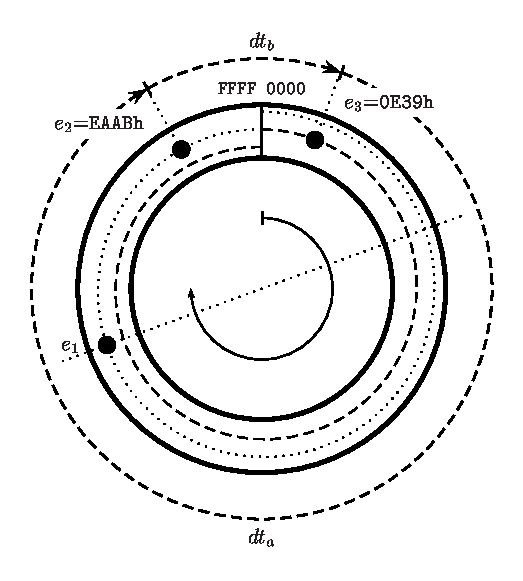
\includegraphics[width=10cm]{images/ictoh.eps}
\end{center}
\caption{The relative timer representation. In the figure, $e_2$ comes before $e_3$}
\label{fig:ictoh}
\end{figure}

The approximation in general is quite good, because it allows to
handle the common cases of periodic tasks with deadline spanning from
a few milliseconds to hundreds of microseconds. with a relatively good
precision.




\pagebreak

\begin{function}{GetTime}
  \synopsis{TimeAbsType GetTime(void);}
  \begin{fundescription}
    This function is used to return the current system time.  This
    function is typically called inside a task, inside the main task
    or inside a ISR type 2.
  \end{fundescription}
  \begin{funreturn}
    \fret{TimeAbsType}{The current timer value.}
  \end{funreturn}
  \begin{funconformance}
    EDF
  \end{funconformance}
\end{function}

%%%%%%%%%%%%%%%%%%%%%%%%%%%%%%%%%%%%%%%%%%%%%%%%%%%%%%%%%%%%%%%%%%%%%%


%%%%%%%%%%%%%%%%%%%%%%%%%%%%%%%%%%%%%%%%%%%%%%%%%%%%%%%%%%%%%%%%%%%%%%

\section{System Startup}
When using the minimal API, there is no need a specific startup
procedure. In particular, the kernel is already active after the first
instruction of the \fn{main} function.

A typical application will be structured with application dependent
initialization routines inside the \fn{main} function. Then, tasks
will be activated with calls to \reffun{ActivateTask}, and finally the
\fn{main} task will end with a forever loop, implementing in this way
the background task.
